\gobbletocpage
\chapter{Testing Ecotype Simulation 2}
\restoretocpage

\begin{shadequote}
I wanna make sure you're ready, brother. Here it is: Show me the money. Oh-ho-ho! SHOW! ME! THE! MONEY! A-ha-ha! Jerry, doesn't it make you feel good just to say that! Say it with me one time, Jerry. \par\emph{Rod Tidwell}
\end{shadequote}


\section{Methods}
The methods chosen for testing were based on a previous study~\cite{carlo}, with few modifications.
Our main goals were to test ES2's accuracy for small input sizes, large input sizes, and show ES2's speed improvements over ES1, involving many \emph{in silico} or computer generated dataset tests and a test of ES2 on previous \emph{Bacillus} data samples from Death Valley.

To test the accuracy of different algorithms we utilized an established pipeline~\cite{carlo}, (see Figure~\ref{fig:ComparisonFlow} on page~\pageref{fig:ComparisonFlow}) which involves generating sequences, and a corresponding demarcation answer key in a standard format.
The generated sequences are then passed through all the demarcators, including a random demarcator (used as a control), producing clustering output in the established standard format.
We then use a metric (Variation of Information) to compare each resulting output to the corresponding answer key that gives a quantification for accuracy. Figure~\ref{fig:ComparisonFlow} on page \pageref{fig:ComparisonFlow} clearly shows the workflow for this pipeline.

Speed tests were done using the python `time' package to clock starting and finishing times of each algorithm for several repetitions, finding the mean running time on various datasets~\cite{carlo}.

\begin{figure}[h!]
\centering
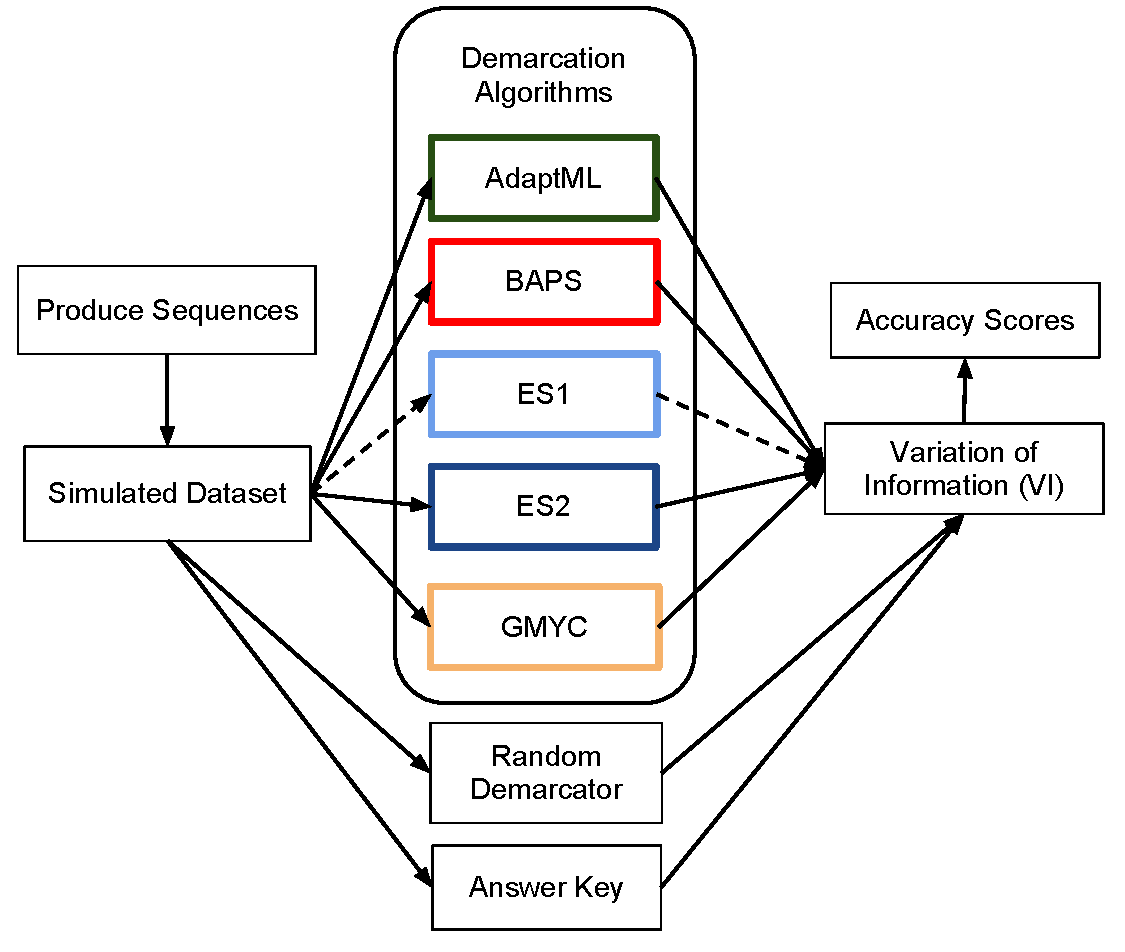
\includegraphics[scale=0.75]{images/DemarcationComparisonsFlow-CH4}
\caption[Demarcation comparison flow diagram.]{A flow diagram for the running of demarcation accuracy comparisons. The produce sequences program takes variable parameters and makes simulated datasets that are used as inputs for various demarcation algorithms, the random demarcator, and answer key generation. Answer keys are generated directly from the knowledge involved in producing the sequences i.e., we know \emph{a priori} which strains belong in an ecotype and how many total ecotypes there are. All the resulting output is compared against the answer key with the Variation of Information (VI) metric to determine accuracy. The dotted line is present because ES1 is not run on the larger datasets.}
\label{fig:ComparisonFlow}
\end{figure}

\subsection*{Other demarcation algorithms}
As a rite of passage, we compare ES against other available demarcation algorithms~\cite{carlo}.
Previously, ES was demonstrated to be the most accurate, yet slowest demarcator.
ES2 aims to be just as accurate as ES1 but a lot faster, enabling larger input size functionality.
The other demarcation programs currently available utilize a variety of clustering models.

\subsubsection*{GMYC~\cite{barraclough2009inferring}}
The GMYC algorithm assumes a Yule model of speciation followed by a neutral coalescent model within species, where drift is the only process yielding coalescence.
It was originally designed to delineate species from sequences for sexually reproducing organisms such as insects, but later was shown to be applicable to asexually reproducing organisms.
GMYC needs only an ultrametric phylogentic tree to demarcate strains.
It is available as a part of the SPLITS package installed and imported onto any local R environment on Mac, Linux, and Windows.
In some tests GMYC had difficulty with generated trees.

\subsubsection*{BAPS~\cite{corander2007bayesian}}
The Bayesian Analysis of Population Structure (BAPS) application refines existing Bayesian approaches to determine the structure of populations from genetic data.
It assumes a partition-based mixture model and performs classification using a variant of the Metropolis-Hasting algorithm to identify clusters of sequences, with no explicit model of purging diversity within clusters.
However, the algorithm can take into account recombination within and between populations.

BAPS has Windows, Linux and Mac versions with GUIs and a command line interface designed for batch processing (this feature does not function in the Mac platform).

\subsubsection*{AdaptML~\cite{hunt2008resource}}
AdaptML places strains into ecotypes based on the assumption that the origin of each ecotype is driven by a change in habitat preferences.
Unlike the cohesion-based algorithms, it only requires a phylogentic tree and data specifying habitat isolation measurements for each strain.
The algorithm assumes a hidden Markov model for the evolution of habitat association and maximizes the likelihood of associations of the strains observed on the tree.

AdaptML runs on any operating system with a  version of Python installed. There is also a web app version of the algorithm where one can upload the data set and have AdaptML demarcations emailed.

\subsubsection*{Random demarcation}
I developed a random demarcator to serve as a control.
In it I picked a random number between one and the number of samples as the $npop$ value (we also experimented with variations of $npop$ choices, including using the correct $npop$). 
Then I randomly distributed the generated sequences throughout $npop$ ecotypes using the broken-stick model~\cite{tokeshi1990niche}, and finally wrote a demarcation output file (see Figure~\ref{code:RandomDemarcating} on page~\pageref{code:RandomDemarcating}).

%Previous figure of code
%\begin{figure}[h!]
%\centering
%\noindent\code{Random Demarcation}{code/random_formatted.py}
%\caption[Python code showing a random demarcator.]{A description with more to be added soon, code needs to be cleaned up.}
%\label{code:RandomDemarcating}
%\end{figure}

\begin{figure}[h!]
\begin{algorithm}[H]
 \SetAlgoLined
% \KwData{c1 is a cluster of sequences, c2 is another cluster of sequences, seq-dist is a function that takes two sequences and returns the distance between them}
% \KwResult{the distance between two clusters}
\SetKwInOut{Input}{input}\SetKwInOut{Output}{output}

\Input{$sequences$ to be demarcated}
\Output{random demarcation based on broken stick distribution}
\BlankLine
 $randomNpop \gets $chooseNpop$(sequences)$\\
 $ecotypeDistribution \gets $[$|sequences|$]\\
 \While{$|ecotypeDistribution| \neq randomNpop$} {
 shuffle$(ecotypeDistribution$)\\
 $chosenEcotype \gets $pop$(ecotypeDistribution)$\\
 \If {$chosenEcotype \neq 1$} {
 $newEcotype1 \gets $random int between 1 and $(chosenEcotype - 1)$\\
 $newEcotype2 \gets chosenEcotype - newEcotype1$\\
 add $newEcotype1$ and $newEcotype2$ to $ecotypeDistribution$\\
 }
 }
 $ecotypes \gets \emptyset$\\
 shuffle$(sequences)$\\
 \For{$n \in ecotypeDistribution$} {
 add [$n$ popped individuals from $sequences$] to $ecotypes$\\
 }
 Write $ecotypes$ to output demarcation file\\
\end{algorithm}
\caption[Pseudocode showing a random demarcator.]{Pseudocode for the random demarcation algorithm. First a function is called to choose $npop$ (a separate function so we can easily modify how we choose $npop$ for variations of the algorithm). Then we form an ecotype distribution structure that has an integer entry per ecotype representing the number of sequences in the ecotype. We randomly choose an ecotype to split into two separate ecotypes (known as the broken-stick algorithm) until we have the same number of ecotypes as chosen $npop$. Finally, we distribute sequences according to the established ecotype distribution, and write the output file.}
\label{code:RandomDemarcating}
\end{figure}


\subsection*{Generation of sequences for analysis}
In order to compare the accuracy of several demarcation programs, the true parameters of the test data must be known.
The problem can be summarized as generating a history for a monophyletic group of $x$ organisms.
Clade history was based on an ecotype formation rate ($\Omega$), the rate of periodic selection ($\sigma$), and the number of ecotypes (\emph{npop}) within the sample.
We used the Ecotype Simulation algorithm to generate each organism's sequence and ecotype affiliation.
Habitats were indicated by either an ``A'' or ``B'', and favored habitat switches with each ecotype formation.
We generated datasets with differing numbers of simulated sequences, and based them on three values each of $\Omega$ and $\sigma$.
The middle values of $\Omega$ and $\sigma$ were 0.19 and 1.1 respectively, based on prior ES analysis of \emph{Bacillus} isolates from a Death Valley canyon~\cite{connor2010ecology}.
Lower and upper values represented a difference of a factor of 10 of the \emph{Bacillus} values.
$Npop$ values were chosen based on the specific run's input size.
We generally tried to choose $npop$ values of 10, 30, and 40 percent regarding input size.

\subsubsection*{Preparing the input}
PhyML~\cite{guindon2010new}, a maximum likelihood tree construction algorithm, was used to build a phylogenetic tree from generated sequences.
The tree was converted into an ultrametric chronogram using Sanderson's nonparametric rate smoothing algorithm, which is included in the APE package.
This ultrametric tree was used as input for GMYC.

AdaptML requires habitat information from which each strain was isolated.
In previous studies we designed a specialization metric for designating habitats, however we found a specific unit of this metric that worked best~\cite{carlo}.
Thus, we will focus on using the best parameter of habitat specialization for AdaptML analysis, and include one other value of specialization (20).

FASTA sequences were converted into XLS format for compatibility with the BAPS package.

\subsection*{Variation of Information Metric}
The Variation of Information (VI) metric~\cite{meilua2003comparing} was used as a criterion for comparing two partitions of the same data set, in order to determine the closeness of each algorithm's ecotype demarcations to the canonical demarcations generated \emph{in silico}.
The Variation of Information between two clusterings C and C' is given by$$VI(C, C') = H(C) + H(C') - 2I(C, C')$$where H(C) is the entropy of a random variable associated with a sequence being in a cluster C and I(C,C') is the mutual information of the two associated variables. 
The important relationship to keep in mind is that the lower the VI score the more accurate the demarcation.

\subsection*{ES2 on smaller datasets}
I ran the new and improved ES2 algorithm on generated datasets for parameters clearly defined in previous studies~\cite{carlo}.
All sample datasets included fifty sequences, and were repeated ten times to find the mean VI score (see Figure~\ref{fig:ESvES2} on page~\pageref{fig:ESvES2}). Also, on a few specific values we ran ES1 and ES2 through one hundred repetitions to find more robust VI scores.

\subsubsection*{Bacillus sequences}
\emph{Bacillus} strains were isolated from Radio Facility Wash, a west-running canyon in Death Valley, consisting of habitats with three levels of solar exposure, including the canyon's sunny south-facing slope, the shadier and cooler north-facing slope, and the arroyo at the bottom~\cite{connor2010ecology}.
Solar exposure habitats served as the only ecological dimension used for environmental input into AdaptML.
Sequences were processed as previously reported~\cite{carlo}.
Again we used PhyML to produce a maximum likelihood tree.

\subsection*{All demarcation programs on large datasets}
We ran all working demarcation programs, and a random demarcator on generated datasets of 50 (see Figure~\ref{fig:All50} on page~\pageref{fig:All50}), 100 (see Figure~\ref{fig:All100} on page~\pageref{fig:All100}), and 200 (see Figure~\ref{fig:All200} on page~\pageref{fig:All200}) sequences.
Parameters were once again adopted from previous studies.
The exception being a choice of $npop$ which, was three values of 10, 20, 30, 40, 50.
We tried to pick $npop$ values that would hit the sweet spot of demarcation performance in addition to an upper and lower bound (i.e., regarding VI accuracy scores).

\subsection*{Running Time Tests}
We tested the running time of each algorithm on a 2.66GHz Intel Core 2 Duo processor with 4GB of RAM running Windows 7.
We present the mean run times that each algorithm required to analyze synthetic data sets constructed using the parameter values estimated previously for \emph{Bacillus}, with various input sizes, and at least 5 repetitions.

\section{Results and Discussion}

%Proof of concept for a figure!
%\begin{figure}[h!]
%  \caption[Demarcation comparison table for small inputs (nu = 50).]{A comparison table of all demarcation algorithms run with differing sigma, omega, and npop values on input sizes of 50 sequences. Parameter combinations in which ES2 outperformed ES1 are circled in red. [I probably won't put in the full table, but parts of it and leave the big one for the appendix]}
%  \centering
%    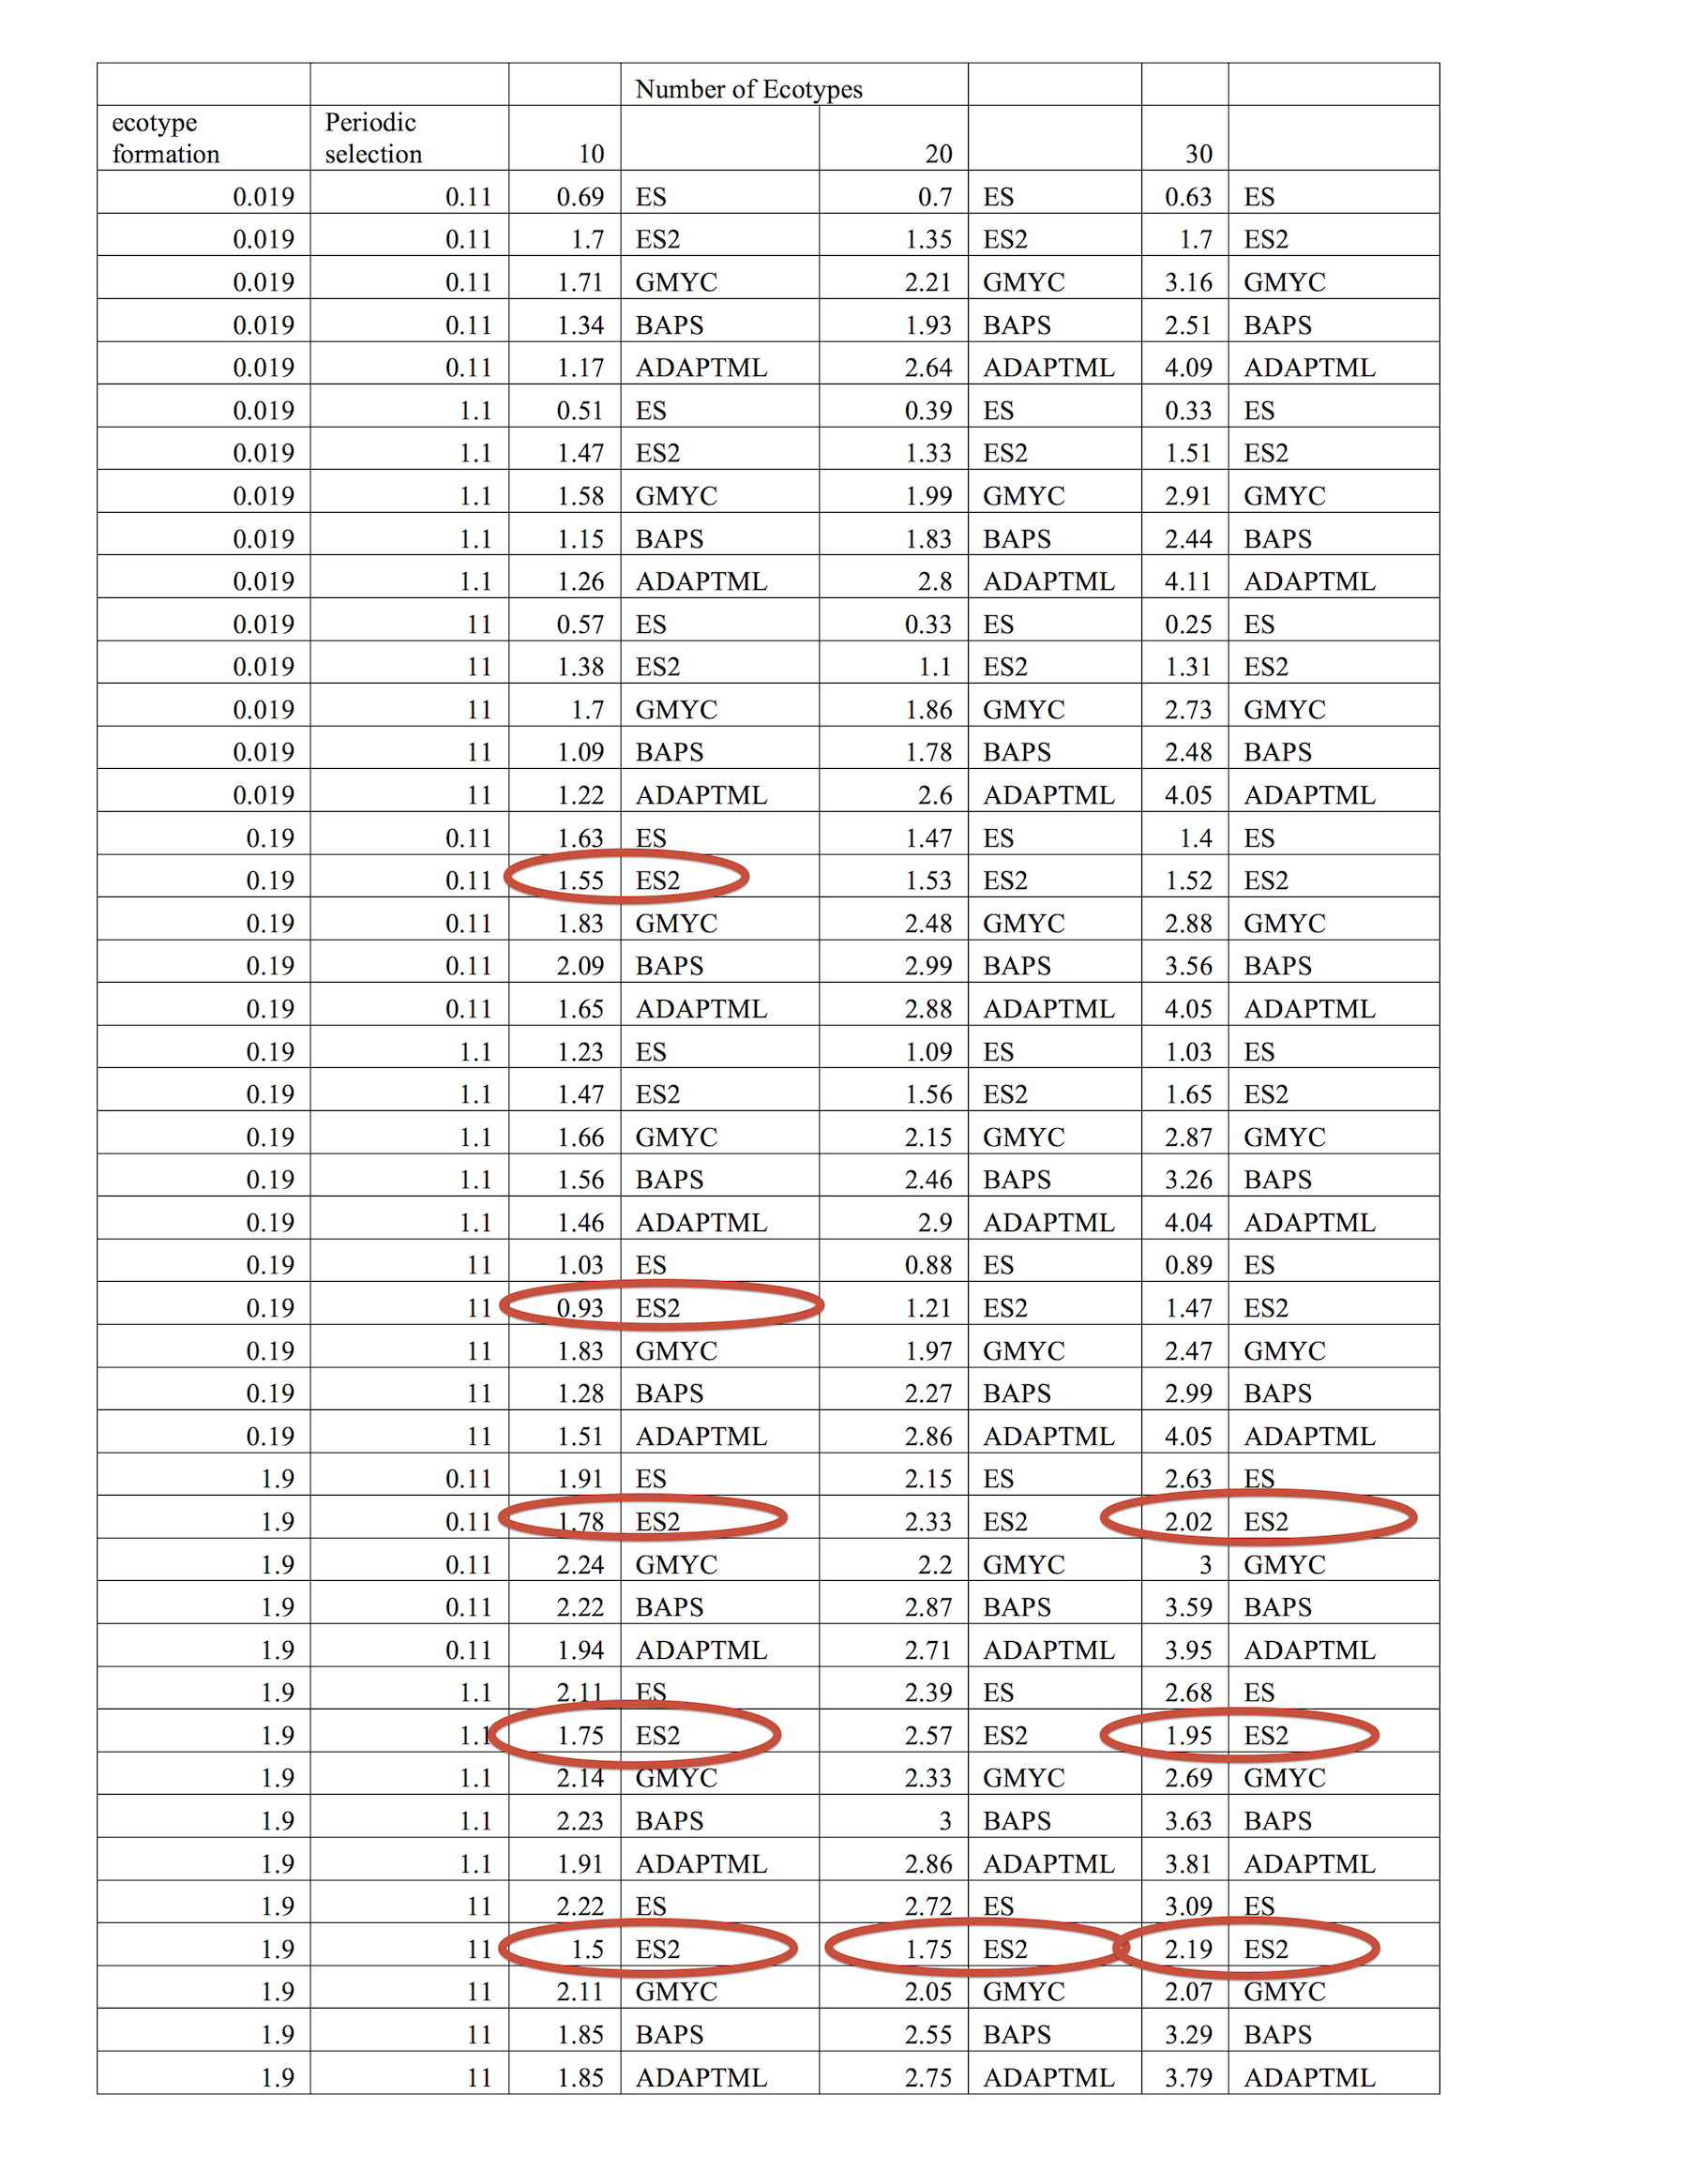
\includegraphics{images/ComparisonTable1.png}
%    \label{fig:ComparisonSmall}
%\end{figure}

\subsection*{Analysis of in silico-generated sequences}
The majority of my work was putting together a dataset of in silico generated sequences demarcation runs.
%A lot of the code I used to run tests was legacy code from past lab members.
I used legacy code from previous lab members as part of this work, after updating dependency packages and modifying certain portions to function on various computer platforms.
%I had to update many dependency packages, and modify certain portions to work on various computer platforms.
As mentioned, BAPS's batch mode does not run on Macintosh.
GMYC worked half of the time, and other times there were errors based on tree generation.
Some analysis does not include GMYC due to this unresolved issue.

\subsubsection*{ES2 on smaller datasets}
Our first experiment was to run Ecotype Simulation (ES) and Ecotype Simulation 2 (ES2) on smaller (i.e., $nu = 50$) datasets (see Figure~\ref{fig:ESvES2}).
%Nested npop, omega, sigma
\begin{figure}[h!]
  \centering
    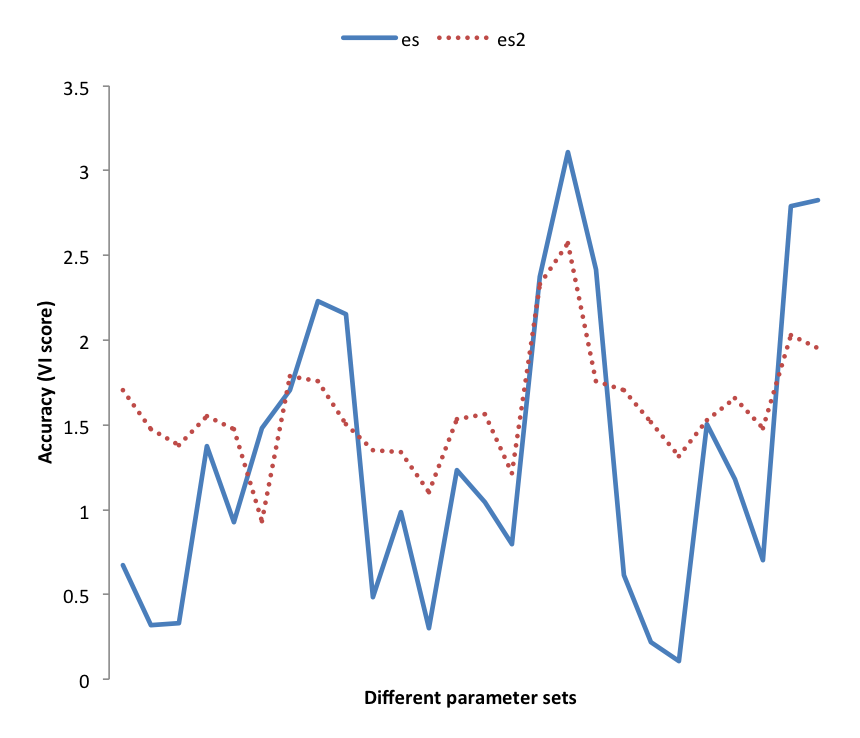
\includegraphics[scale=0.75]{images/ResultGraphs/ResultGraphs-4}
      \caption[ES vs ES2 accuracy visualization on $nu = 50$.]{Across 27 parameter set combinations I exhaustively tested ES (solid line) and ES2 (dotted line) on $npop$ values of 10, 20, and 30, $\Omega$ values of 0.019, 0.19, and 1.9, $\sigma$ values of 0.11, 1.1, and 11, for nu of 50 sequences. The nested parameter loop is represented for one triple of values below the $x$-axis. The subsequent parameter test points cycle logically through medium and high omega values and then medium and high $npop$ values. All following graphs similar to this one use the same parameter scheme. On the $y$-axis we have VI scores, where values closer to 0 represent more accurate demarcation runs.}
    \label{fig:ESvES2}
\end{figure}
Notice how close the two lines are over all the parameters.
ES1 (solid line) is generally lower (i.e., more accurate), however there are dramatic peaks and valleys of performance.
In contrast to ES2 (dotted) which overall was quite accurate with few valleys and peaks.
\begin{table}
    \begin{tabular}{l|cc}
    ~                  & Ecotype Simulation & Ecotype Simulation 2 \\ \hline
    Average            & 1.30414053         & 1.596300918          \\
    Standard Deviation & 0.877454163        & 0.343838045          \\
    \end{tabular}
    \caption[ES versus ES2 statistics.]{Statistics on the ES vs ES2 run with 10 reps on a dataset of $nu=50$.}
    \label{tab:ESvES2mean}
\end{table}
This trend is represented in Table~\ref{tab:ESvES2mean} on page~\pageref{tab:ESvES2mean}, by ES2's lower standard deviation than ES1.
However, ES1 still has a lower mean VI score, but not by much.
We also chose 3 canonical parameters (\emph{Bacillus} values with varying omega) to run ES1 and ES2 on 100 repetitions.
Results in raw form for this experiment can be found in Figure~\ref{fig:HundredResultsFile} in the Appendix.
Surprisingly, ES2 outscored ES1 in the 10x omega value parameter run.

From these tests, we are confident about ES2's accuracy.
Across various parameters ES2 looks to be more consistent than even ES1, even though ES1 demarcation often matches the answer key more closely.
On small datasets speed is not such an issue, but if you want to run a lot of small datasets, then we advise using ES2.

\subsubsection*{All demarcation programs on large datasets}
Time becomes a significant issue when we run Ecotype Simulation on datasets of 50 sequences (runtime is \textasciitilde2390 seconds from Table~\ref{tab:ES1speed} on page~\pageref{tab:ES1speed}) or larger.
For this reason we developed ES2 to run on datasets with more than 50 sequences.
From past studies we have found ES to be the most accurate demarcation program~\cite{carlo}, and we expect similar levels of accuracy from ES2 on larger datasets.

%\begin{figure}[h!]
%  \centering
%    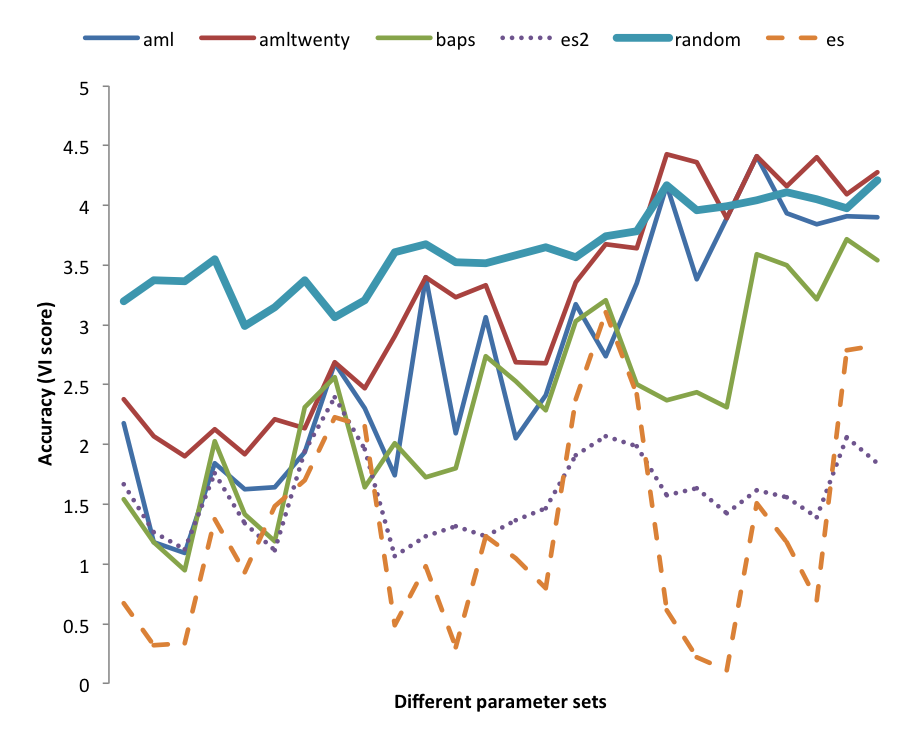
\includegraphics[scale=0.75]{images/ResultGraphs/ResultGraphs-3}
%      \caption[All demarcation graphical accuracy visualization on $nu = 50$.]{Across 27 parameter set combinations I exhaustively test all demarcation programs on $npop$ values of 10, 20, and 30, $\Omega$ values of 0.019, 0.19, and 1.9, $\sigma$ values of 0.11, 1.1, and 11, for nu of 50 sequences. Random demarcation is represented by the solid line. On the $y$-axis we have VI scores, where values closer to 0 represent more accurate demarcation runs.}
%    \label{fig:All50}
%\end{figure}
%
%\begin{table}
%    \begin{tabular}{l|ccccc}
%    ~                  & AdaptML     & AdaptML$^\ast$    & Baps        & Ecotype Simulation 2 & Random      \\ \hline
%    Average            & 2.767371639 & 3.185623443 & 2.359650359 & 1.589546505          & 3.631545086 \\
%    Standard Deviation & 0.971373851 & 0.868775294 & 0.783228066 & 0.34336826           & 0.34949857  \\
%    \end{tabular}
%    \caption[Statistics on all demarcators on $nu=50$.]{Statistics on all demarcators run with 5 reps on a dataset of $nu=50$.}
%        \label{tab:50Allmean}
%\end{table}

\begin{figure}[h!]
  \centering
    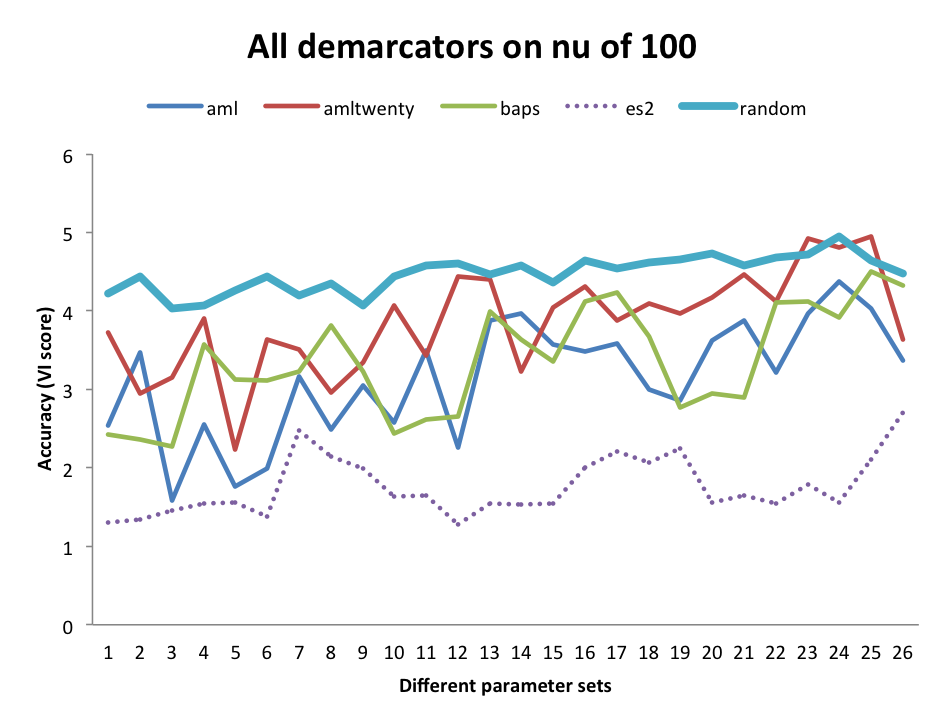
\includegraphics[scale=0.75]{images/ResultGraphs/ResultGraphs-2}
      \caption[All demarcation graphical accuracy visualization on $nu = 100$.]{Across 27 parameter set combinations I exhaustively tested all demarcation programs on $npop$ values of 30, 40, and 50, $\Omega$ values of 0.019, 0.19, and 1.9, $\sigma$ values of 0.11, 1.1, and 11, for nu of 100 sequences. The same parameter scheme was used as with the last similar graph; in this case it was represented implicitly. Random demarcation is represented by the solid line. On the $y$-axis we have VI scores, where values closer to 0 represent more accurate demarcation runs.  ($^\ast$) Represents AdaptML ran with a habitat specialization value of 20.}
    \label{fig:All100}
\end{figure}

Figure~\ref{fig:All100} on page~\pageref{fig:All100} shows accuracy scores for all demarcating programs on a variety of parameters (\emph{Bacillus} values with .1x and 10x and $npop$ values of 30, 40, 50) on sample size of 100 individuals.
Notice that overall ES2 (dotted line) was the lowest (i.e., most accurate), signifying ES2's demarcation output matched most closely to the answer key demarcations.
This fact is highlighted by the lowest average VI score shown in Table~\ref{tab:100Allmean}, of 1.76.
Also, notice that once again ES2 has the lowest standard deviation, meaning that it was the most consistent, except for the random demarcation, which performed poorly (as we would expect).
ES2 (accuracy) was followed by AdaptML (3.14), BAPS (3.36), and Random (4.47).

ES2 appeared to be slightly more accurate with higher $npop$ values; the gap between it and other demarcators increased.
Higher rates of $\Omega$ (rate of ecotype formation) resulted in slight increases in ES2's VI scores.
It appears that changes in $\sigma$ (rate of periodic selection) did not affect the accuracy of each algorithm as much as modifying $\Omega$.
$Npop$ appears to have had the greatest effect on the accuracy of all the demarcation programs, least of all ES2.
Losing accuracy with greater values of $npop$ was a trend that continued with larger datasets (see supplementary figures in Appendix).

\begin{table}[h!]
%    \begin{tabular}{l|ccccc}
%    ~                  & AdaptML     & AdaptML$^\ast$     & BAPS        & Ecotype Simulation 2 & Random      \\ \hline
%    Average            & 3.142555041 & 3.860006018 & 3.363530792 & 1.762829323          & 4.475184564 \\
%    Standard Deviation & 0.727870506 & 0.639625177 & 0.67100242  & 0.370748481          & 0.225368714 \\
%    \end{tabular}
    \begin{tabular}{l|cc}
    ~                    & Average     & Standard Deviation \\ \hline
    AdaptML              & 3.142555041 & 0.727870506        \\
    $^\ast$AdaptML              & 3.860006018 & 0.639625177        \\
    BAPS                 & 3.363530792 & 0.67100242         \\
    ES 2 & 1.762829323 & 0.370748481        \\
    Random               & 4.475184564 & 0.225368714        \\
    \end{tabular}
    \caption[Statistics on all demarcators on $nu=100$.]{Statistics on all demarcators run with 5 reps on a dataset of $nu=100$. ($^\ast$) Represents AdaptML ran with a habitat specialization value of 20. }
        \label{tab:100Allmean}
\end{table}

Tests regarding large datasets are ongoing.
In the Appendix there are additional graphs with all demarcators run on nu of 50 and 200 along with corresponding tables showing mean and standard deviation values.
These tests were done only 5 repetitions, so far.
We would like repetitions in the hundreds.

%
%\begin{figure}[h!]
%  \centering
%    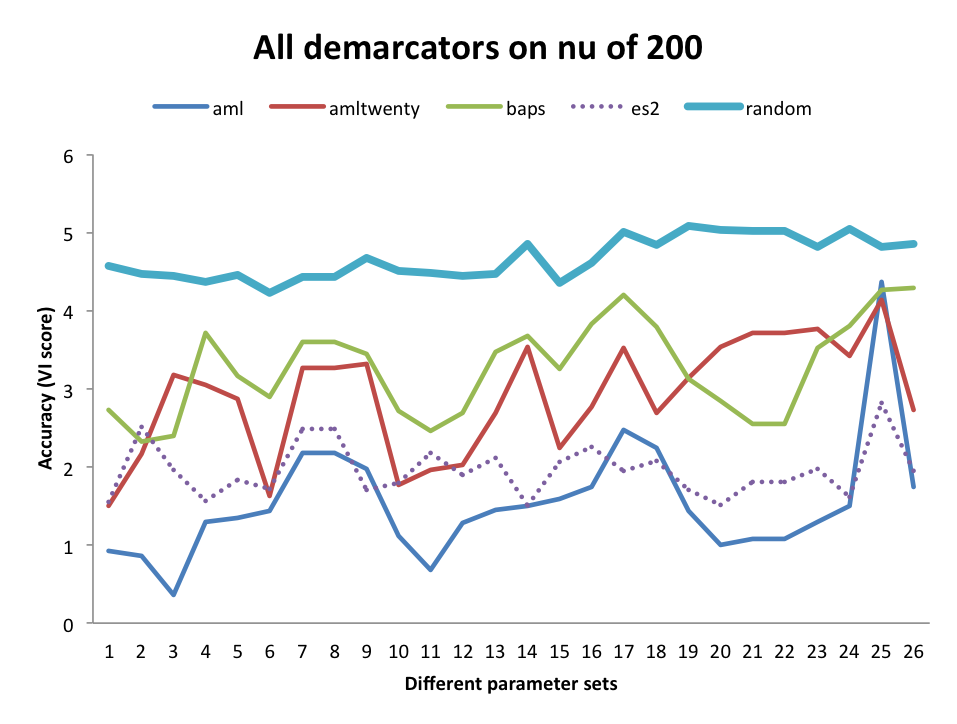
\includegraphics[scale=0.75]{images/ResultGraphs/ResultGraphs-1}
%      \caption[All demarcation graphical accuracy visualization on $nu = 200$.]{Across 27 parameter set combinations I exhaustively test all demarcation programs on $npop$ values of 30, 40, and 50, $\Omega$ values of 0.019, 0.19, and 1.9, $\sigma$ values of 0.11, 1.1, and 11, for nu of 200 sequences. Random demarcation is represented by the solid line. On the $y$-axis we have VI scores, where values closer to 0 represent more accurate demarcation runs.}
%    \label{fig:All200}
%\end{figure}
%
%\begin{table}
%    \begin{tabular}{l|ccccc}
%    ~                  & AdaptML     & AdaptML$^\ast$     & BAPS        & Ecotype Simulation 2 & Random      \\ \hline
%    Average            & 1.543424394 & 2.908133924 & 3.265003881 & 1.955714164          & 4.667531001 \\
%    Standard Deviation & 0.748104722 & 0.713876097 & 0.59283446  & 0.33348659           & 0.258112685 \\
%    \end{tabular}
%    \caption[Statistics on all demarcators on $nu=200$.]{Statistics on all demarcators run with 5 reps on a dataset of $nu=50$.}
%        \label{tab:200Allmean}
%\end{table}

\subsection*{\emph{Bacillus} sequences}
I ran ES2 on \emph{Bacillus} sequences from previous studies.
The results were consistent with previous demarcation runs (see Figure~\ref{fig:Bacillus} on page~\pageref{fig:Bacillus}).
ES2's demarcations followed ES's closely.
There was an instance where ES2 found two distinct ecotypes where ES only found one; matching GMYC's cluster boundary.
Yet, there was another instance where two discrete ES ecotypes were grouped together.
Results on \emph{Bacillus} sequences are within the bounds of what we would expect to see from a demarcation algorithm.
ES2 passed the \emph{Bacillus} sanity check.

\begin{figure}[h!]
  \centering
    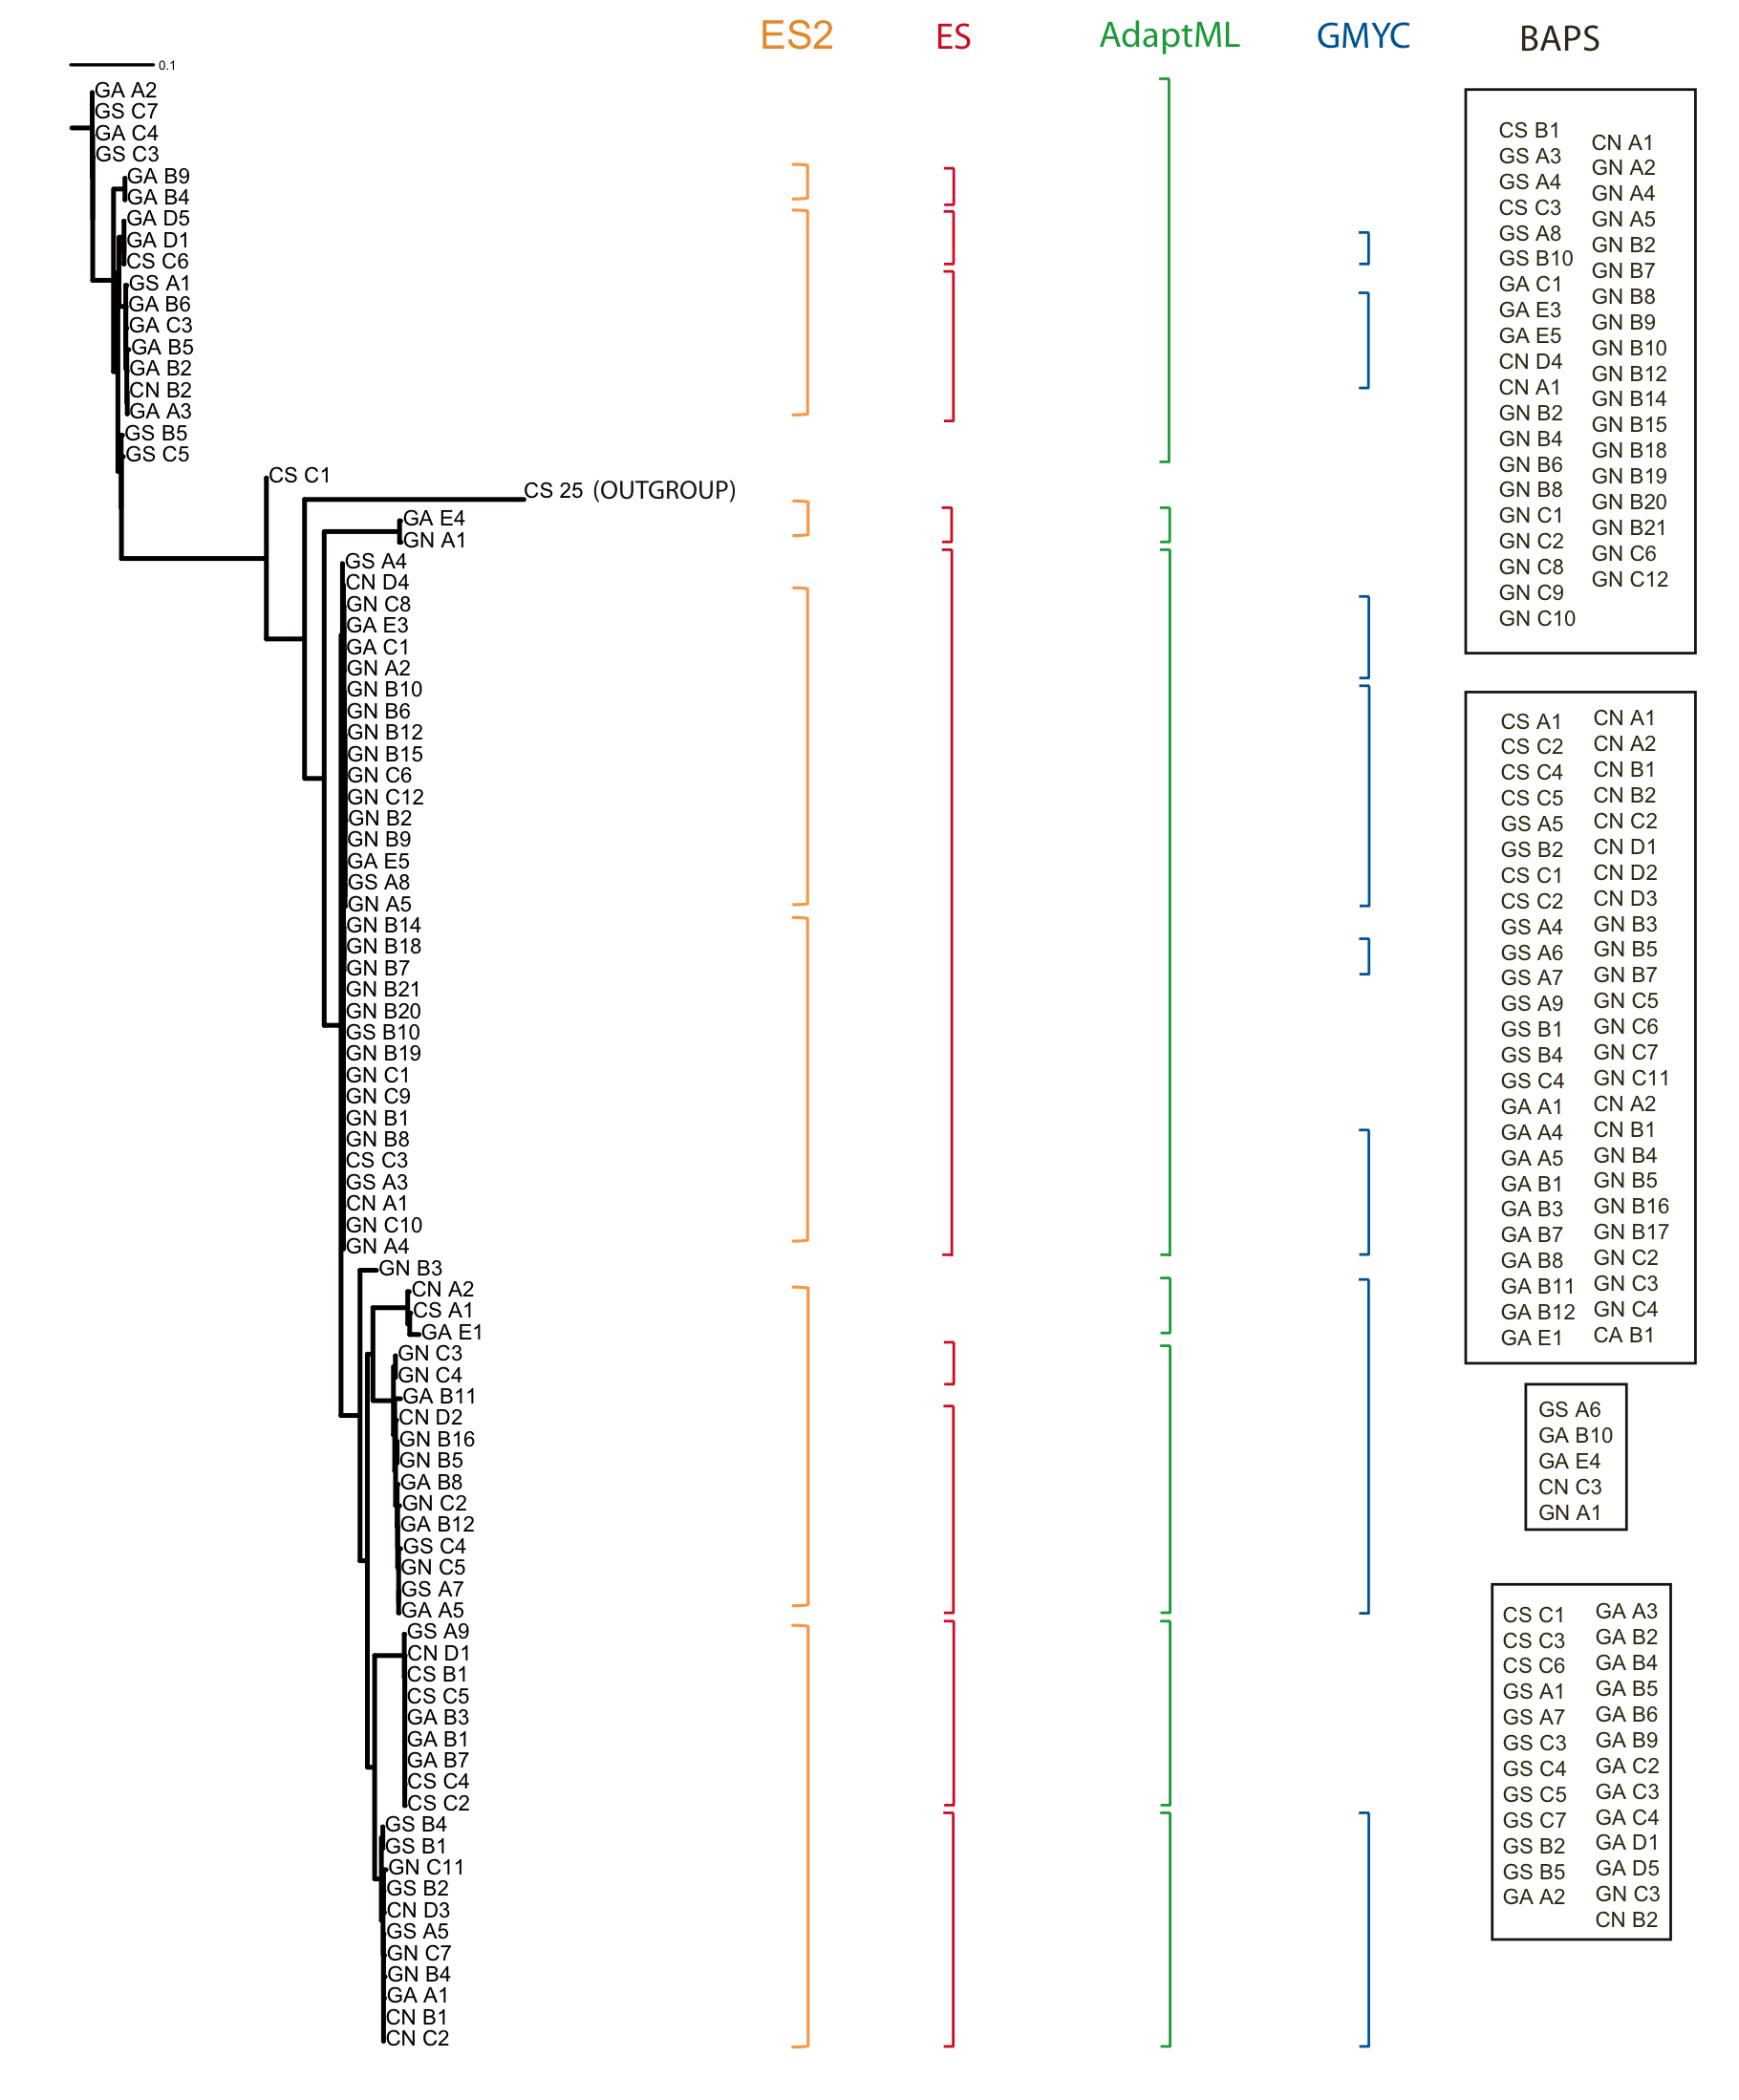
\includegraphics[scale=0.4]{images/Bacillus-CH4}
      \caption[Demarcation programs run on previous \emph{Bacillus} sequences.]{Demarcation programs run on previous \emph{Bacillus} sequences. ES2 (orange) found 7 distinct ecotypes and multiple singletons (not included here). The other demarcation results are from previous runs on the same input set. (adapted from~\protect\cite{carlo})}
    \label{fig:Bacillus}
\end{figure}

\begin{figure}[h!]
  \centering
    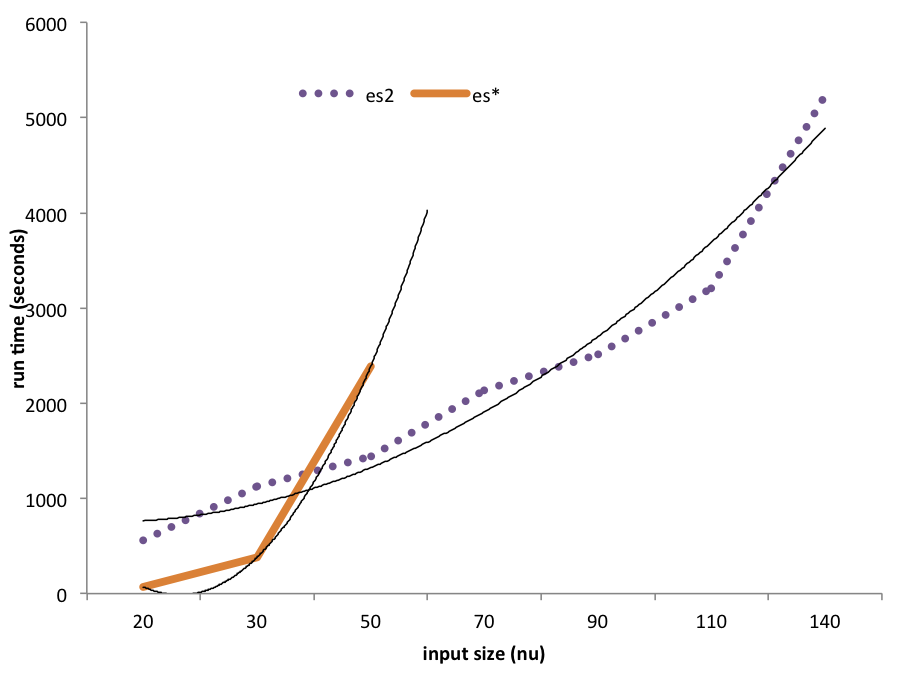
\includegraphics[scale=0.7]{images/SpeedWindows-CH4}
      \caption[Demarcation run time test on Windows.]{Comparison of demarcation runtimes on a Windows. The dotted line represents ES2's runtime. Most demarcators run completely within seconds.}
    \label{fig:WindowsSpeed}
\end{figure}

\begin{table}
\centering
    \begin{tabular}{l|cccccc}
    Algorithm & 20   & 30    & 50     & 110    & 140    & 170    \\ \hline
    AdaptML   & na   & 2.0   & 3.0    & 5.0    & 5.4    & 5.8    \\
    BAPS      & na   & 9.0   & 15.3   & 26.8   & 28.7   & 34.3   \\
    ES1       & 69.8 & 384   & 2390   & na     & na     & na     \\
    ES2       & na   & 558.7 & 1127.4 & 2511.5 & 3208.0 & 5237.2 \\
    \end{tabular}
    \caption[Speed testing information on all demarcation algorithms.]{Speed testing information on all demarcation algorithms for various numbers of nu or numbers of sequences. ES2 is faster than ES1 but not faster than the other demarcation algorithms.}
    \label{tab:WindowsSpeed}
\end{table}

\subsection*{Running time}
We compared the running times of the demarcation algorithms on synthetic data sets of different sizes, and found that AdaptML, GMYC, and BAPS performed demarcations much more quickly then ES2 (see Figure~\ref{fig:WindowsSpeed} on page~\pageref{fig:WindowsSpeed}).
AdaptML, GMYC (if it worked), and BAPS all completed demarcations on the order of a few seconds, even for datasets in the hundreds whereas ES2 required on the order of tens of minutes for the same inputs.
AdaptML was the fastest algorithm, taking no more than one second on average; BAPS followed and ES2 was only faster than ES1 (see Table~\ref{tab:WindowsSpeed} on page~\pageref{tab:WindowsSpeed}).
ES1 ran faster than ES2 on an input of size 30 because of the constant speed slow-down incurred by our modified automatic demarcation.
Input sizes with only 20 sequences ran approximately twice as fast in ES2, because the algorithmic modifications began to outweigh demarcation slow down.
We are still working on ways of best evaluating runtime, however it is quite clear that ES2 greatly outperforms ES1 speed wise.

Since the BAPS's batch processing feature was not available for Mac I ran it on Windows.
However, I also ran ES2, GMYC, and AdaptML separately on my Mac and found that ES2 was significantly faster than when it was run on a Windows machine.

\section{Chapter Summary}
In this chapter I discussed the motivation and thought process behind our experiments.
I gave a survey of other available demarcation programs (GMYC, BAPS, AdaptML) and our control random demarcator, how we generated sample datasets, and described the metric used to compare the various outputs (Variation of Information metric).

First we wanted to show that ES1 and ES2 achieve similar levels of accuracy.
Therefore, we ran ES1 and ES2 on data sets with 50 individuals for 10 repetitions.
ES2 achieved comparable accuracy, and had a lower standard deviation.
Next, we ran all the demarcator programs on various sized data sets.
ES2 maintained a high level of accuracy throughout a wide range of parameters (based on previous \emph{Bacillus} values).
Traditionally we run all demarcators on \emph{Bacillus} sequences; ES2 performed well.
ES's previous demarcations were similar, even though their were a few extra ecotypes discovered and in other instances separate ecotypes grouped together.
Once again ES2 was the slowest demarcation algorithm.
However, it improved dramatically on ES1's running times.


